\documentclass[12pt]{article}

\usepackage[a4paper,margin=2cm,top=2cm,bottom=2cm,xetex]{geometry}
\usepackage[utf8]{inputenc}
\usepackage{color,xcolor}
\usepackage{enumitem}
\usepackage{amssymb}
\usepackage{amsthm}
\usepackage{amsfonts}
\usepackage{mathtools}
\usepackage{flexisym}
\usepackage{algorithm}
\usepackage{pdfpages}
\usepackage{algorithmic}
\usepackage{tabularx}
\usepackage{xepersian}
\usepackage{amsmath}
\usepackage{physics}
%\usepackage{mathtools}

\DeclareFontFamily{U}{matha}{\hyphenchar\font45}
\DeclareFontShape{U}{matha}{m}{n}{ <-6> matha5 <6-7> matha6 <7-8>
matha7 <8-9> matha8 <9-10> matha9 <10-12> matha10 <12-> matha12 }{}
%\DeclareSymbolFont{matha}{U}{matha}{m}{n}
%
%\DeclareMathSymbol{\nvartrianglelefteq}{\mathrel}{matha}{"9E}
%\DeclareMathSymbol{\vartrianglelefteq}{\mathrel}{matha}{"9C}

\newcount\HWcnt
\def\ttmp#1#2#3#4#5#6#7#8#9|{\def\Wjob{#9}}%
\expandafter\ttmp\jobname |
\def\ttmp#1#2#3{\global\HWcnt=#2#3}
\expandafter\ttmp\Wjob

\settextfont[Scale = 1.0 ,
             BoldFont = *Bd ,
             ItalicFont = *It ,
             BoldItalicFont = *BdIt ,
             Extension = .ttf
            ]{XB Niloofar}
\ExplSyntaxOn
\cs_set_eq:NN
\etex_iffontchar:D
\tex_iffontchar:D
\cs_undefine:N \c_one
\int_const:Nn \c_one { 1 }
\ExplSyntaxOff
\setdigitfont[Scale = 1.0 ,
             BoldFont = *Bd ,
             ItalicFont = *It ,
             BoldItalicFont = *BdIt ,
             Extension = .ttf
            ]{XB Niloofar}
\renewcommand{\baselinestretch}{1.2}
\pagestyle{empty}

\makeatletter
\def\abj@num@i#1{%
    \ifcase #1\or الف\or ب\or ج\or د\or ه\or و\or ز\or ح\or ط\fi \ifnum #1=\z@ \abjad@zero \fi
}
\renewcommand{\theenumi}{\abjad{enumi}}
\renewcommand{\labelenumi}{\theenumi)}
\long\def\makeHead#1{%
	\begin{center}\large
		\begin{tabular}{@{}p{.33\linewidth}<{\hfill}@{}>{\hfil}p{.33\textwidth}<{}@{}>{\hfill}p{.33\textwidth}@{}}
            \textbf{محاسبات عددی} & & \textbf{سری شمارهٔ 3} \\[.5ex]
            \textbf{نیم‌سال دوم ۱۴۰۱-۱۴۰۲} & &  \textbf{موعد تحویل: #1}\\[.5ex] \hline\hline
		\end{tabular}
	\end{center}\smallskip
%	\def\theenumii{\arabic{enumii}}\def\theenumi{\alph{enumii}}\def\labelenumi{\theenumi)}\def\labelenumii{\theenumii)}%
}

\newcommand{\Rule}{\ \hfill\rule{\linewidth}{0.5pt}\hfill\ \par\vspace*{-2ex}\par}
\newcommand{\DescRule}{\ \hfill\rule{\linewidth}{1pt}\hfill\ \vspace*{-2ex}\par}
\def\rank{\mathop{\mathrm{rank}}\nolimits}

\begin{document}
\makeHead{پاسخنامه تمرین}
\begin{description}
% 	\item{\textbf{سوال 1.}} \input{\jobname-q1.tex}
	
% 	\Rule
	\item{\textbf{سوال ۱.}}
	\\
فرض کنید تابع \( f \) در بازه  \([a, b]\) دو بار مشتق‌پذیر است و \( x_i \)، \( i = 0, 1, \ldots , n\)، نقاط هم‌فاصله در این بازه‌ هستند که \( x_0 = a\) و \( x_n = b\) می‌باشد. اگر \( p(x) \) چندجمله‌ای درون‌یاب
\footnote{interpolation Polynomial}
پیشروی \( f(x) \) باشد، آنگاه \( f''(x) \) را با مقدار \( p''(x) \) تخمین می‌زنیم.
\\
\\
الف) با فرض
\( s = \frac{{x - x_0}}{{h}} \)
و
\( P(s) = f_0 + \Delta f_0 + \frac{{s(s - 1)}}{{2!}}\Delta^2 f_0 + \ldots + \frac{{s(s-1)\ldots(s-n+1)}}{{n!}}\Delta^n f_0 \)
\\
\(p''(x)\)
را محاسبه کنید.
\\
\\
ب) تخمینی برای \( f''(x_0) \) در حالت کلی، با استفاده از جمله اول محاسبه (الف) و با استفاده از دو جمله اول آن ارائه کنید.
	
	\Rule 
	
	\item {\textbf{سوال ۲.}}
	\\
جدول مقادیر زیر را در نظر بگیرید:

\begin{latin}
\begin{table}[H]
  \begin{center}
    \begin{tabular}{c|c c c}
      \textbf{$x$} & $0$ & $1$ & $2$ \\
      \hline
      \textbf{$f(x)$} & 9.90 & 7.94 & 23.00 \\
    \end{tabular}
  \end{center}
\end{table}
\end{latin}

\begin{enumerate}
	\item
	به‌کمک سری تیلور تقریبی از
    $f''(1)$
    ارائه دهید.
	
	\item
	حد بالای خطای این تقریب را به‌کمک خطای سری تیلور به دست آورید.
\end{enumerate}
\textcolor{blue}{حل
\\
\begin{enumerate}
    \item
    عملا فرمولی که با سری تیلور به آن می‌رسیم همان فرمول نقطه میانی‌ای است که به شکل زیر است:
    \begin{align*}
        f^{''}(x_i) &= \frac{f(x_{i + 1}) - 2f(x_i) + f(x_{i - 1})}{h^2} \\
        &= \frac{23 - 2 (7.94) + 9.9}{1^2} = 17.02
    \end{align*}
    \item
    \begin{align*}
        f(x_i + h) + f(x_i - h) &= \text{جملات توان زوج 
        $h$} \\
        &= 2f(x_i) + h^2 f^{''}(x_i) + \frac{h^4}{4!} \times 2 f^{(4)}(\zeta) \xrightarrow{h = 1}  \frac{1}{12} f^{(4)}(\zeta)
    \end{align*}
    کران بالای بدست آمده به ازای 
    $\zeta$
    در بازه 
    $[x_i, x_i + h]$
    برقرار است.
\end{enumerate}
}
	
	\Rule
	
	\item {\textbf{سوال ۳.}}
	می‌دانیم
$ 1.123 < x < 1.124$.
این عدد را تا ۳ رقم اعشار گرد می‌کنیم و نتیجه را برابر با $r$ قرار می‌دهیم. نشان دهید 
$$|x - r| \leq 0.0005$$


پاسخ:

می‌دانیم که 
$1.1230 < x < 1.1240$
برقرار است.  بنابراین در صورت گرد کردن فاصله حداکثر برابر است با
$0.0005$
	
	\Rule
	
	\item {\textbf{سوال ۴.}}
	\\
با استفاده از قضیه تیلور نشان دهید تقریب از مرتبه \(O(h^4)\) برای مشتقات اول تا سوم \(f(x)\) وجود دارد و همچنین
\\
\[ f'(x_i) \approx \frac{{-f_{i+2} + 8f_{i+1} - 8f_{i-1} + f_{i-2}}}{{12h}} \]

\[ f''(x_i) \approx \frac{{-f_{i+2} + 16f_{i+1} - 30f_i + 16f_{i-1} - f_{i-2}}}{{12h^2}} \]

\[ f'''(x_i) \approx \frac{{-f_{i+3} + 8f_{i+2} - 13f_{i+1} + 13f_{i-1} - 8f_{i-2} + f_{i-3}}}{{8h^3}} \]
\\
خطای برشی هر یک از تقریب‌های بالا \(O(h^4)\) است.
	
	\Rule
	
	\item {\textbf{سوال ۵.}}
	\begin{enumerate}
\item \label{second} دستگاه زیر را با روش 
گاوس-سیدل
\footnote{Gauss-Seidel}
حل کنید.
    \begin{center}
        \begin{cases}
          x - 2y = 4\\
          2x + y = 3
        \end{cases}
    \end{center}
\item \label{first} 
دستگاه زیر را با روش 
گاوس-سیدل
حل کنید
\begin{center}
    \begin{cases}
      2x + y = 3 \\
      x - 2y = 4
    \end{cases}
\end{center}
\item 
چرا با آن که دستگاه‌های 
(الف)
و
(ب)
جواب‌های یکسان دارند ولی همگرایی روش تکرار گاوس-سیدل در 
(الف)
و
(ب)
متفاوت است؟
\end{enumerate}
\noindent \hspace{0.5em} * در 
(الف)
و
(ب)
تقریب اولیه را
$x^{(0)} = y^{(0)} = 0$
در نظر بگیرید.

\textcolor{blue}{
حل 
\\
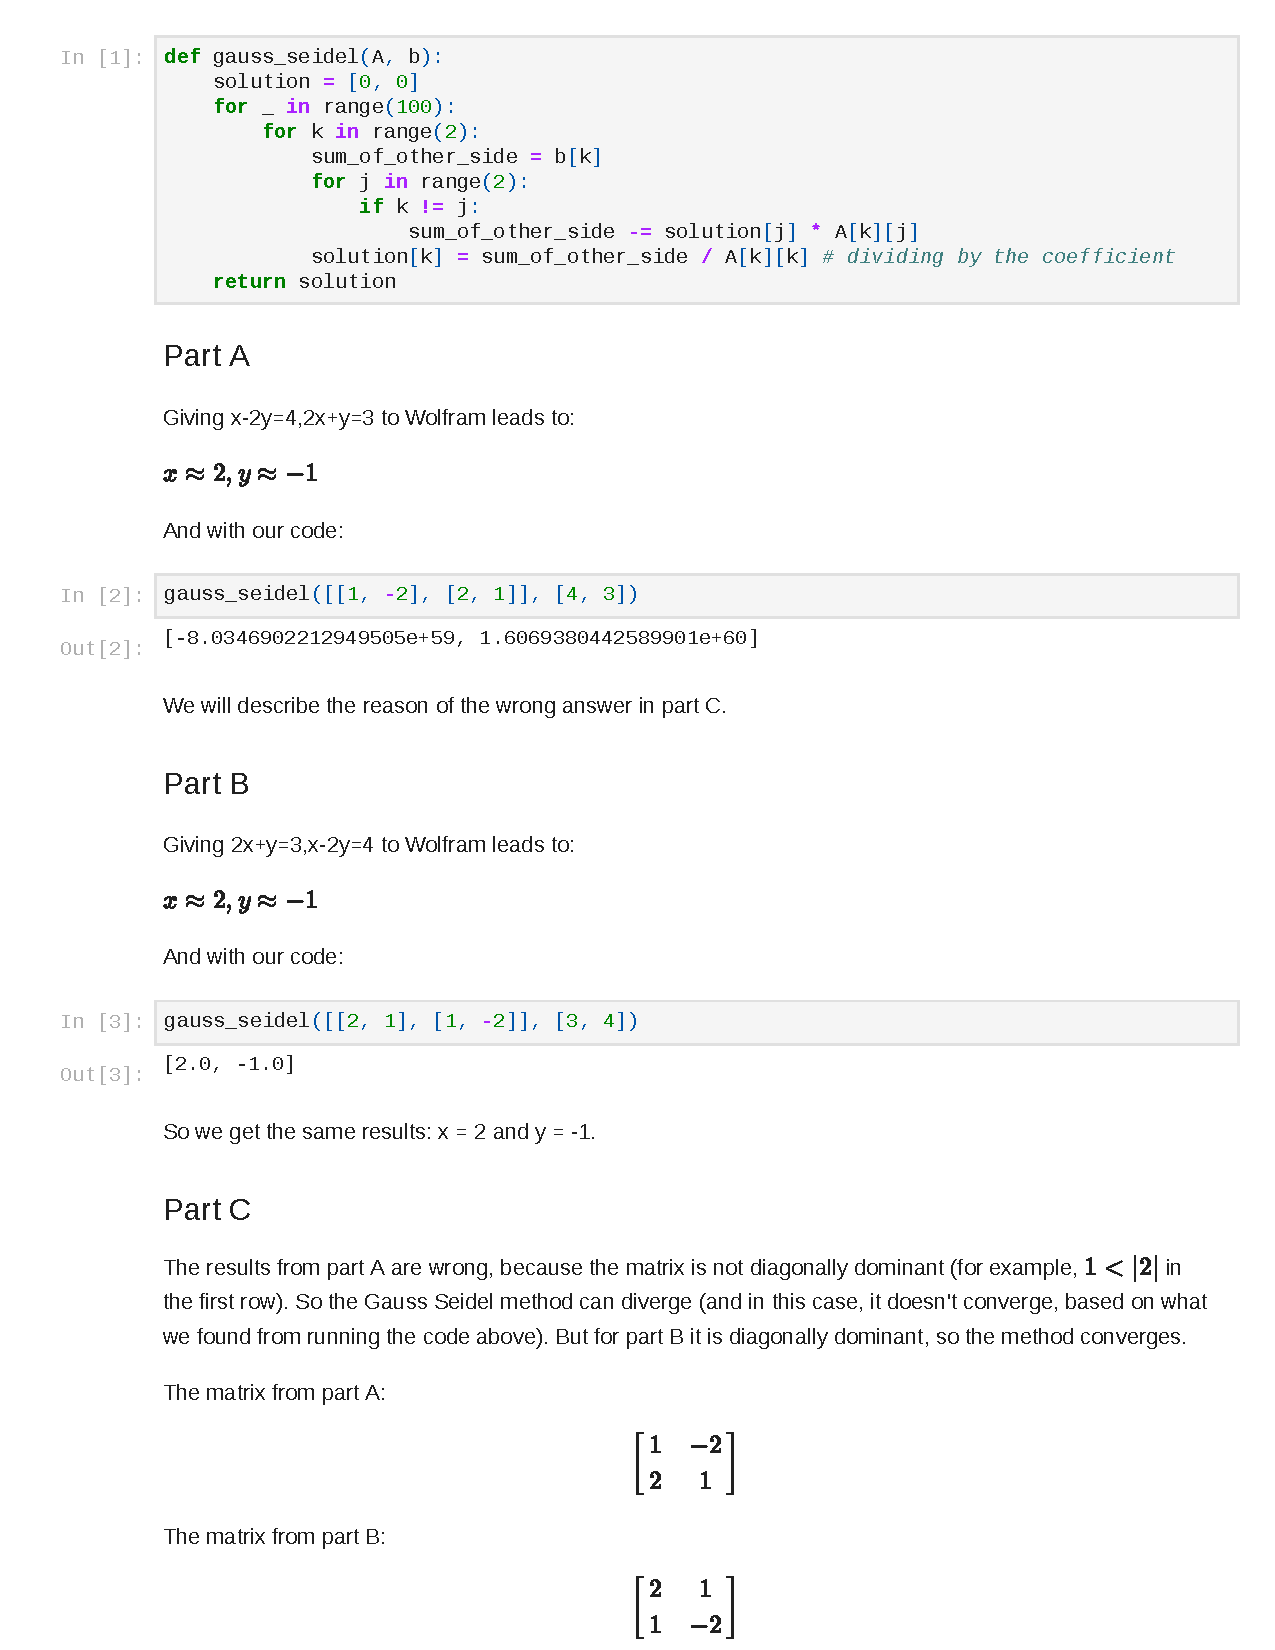
\includepdf[pages={1-},scale=1]{q5.pdf}
}
	
	\Rule

	\vspace*{-2ex}\ \hfill\textbf{موفق باشید.}
\end{description}
\end{document}